\chapter{Objectives and requirements}
\label{cap:requirements}
\intro{In this chapter are discussed the main objectives and requirements.}\\

\section{Cloud Infrastructure}
The system must be able to ingest, store and process large amount of IoT data leveraging the power of at least two cloud providers. Furthermore, the final product must be architectured to be cloud agnostic, meaning that it must be able to run on any cloud provider. This is important because the system must be able to run on different cloud providers to avoid vendor lock-in and to enable the customer to choose the best cloud provider for their needs.\\
For the initial development, the system will be developed using \href{https://aws.amazon.com/it/}{Amazon Web Services}\footcite{site:aws} and \href{https://azure.microsoft.com/it-it/}{Microsoft Azure}\footcite{site:azure} mainly because of the already developed
experience with them, both by the company and by the author of this thesis.

\section{Data collection}
The system must be able to ingest data from online devices and on-premise data sources. 
Online devices are devices that are connected to the internet and can send data to the cloud via MQTT protocol.
On-premise data source are offline files that are stored on a local machine and must be uploaded to the cloud. The system must provide a way to upload these files to the cloud.
\section{Data processing}
The system must be able to preprocess the data before storage. The preprocessing of the data includes data validation, data cleaning and data transformation, this can be done in cloud or on-premise. The system must be also able to process data after storage. The processing of the data includes data analysis and machine learning operations. 

\newpage
\section{Security}
Security is a major concern for the system. In certain scenarios, the data collected could be sensitive and thus must be protected both in transit and at rest.
    \subsection{Security in transit}
    Data in transit are transfered using MQTT protocol which is not encrypted by default. The system must provide a way to encrypt and secure the data in transit. MQTT brokers however supports authentication and authorization through certificates as well as TLS/SSL encryption. Using a broker that supports these features is a must.
    
    \subsection{Security at rest}
    Data at rest is stored in cloud storage. The cloud storage must provide a way to encrypt the data at rest. The system must also provide a way to manage the encryption keys. Both \href{https://aws.amazon.com/it/}{Amazon Web Services}\footcite{site:aws} and \href{https://azure.microsoft.com/it-it/}{Microsoft Azure}\footcite{site:azure} provide a way to encrypt data at rest and manage the encryption keys.\\ 
    Furthermore, both cloud providers uses a shared responsibility model for security.
    
    \newpage
    \subsubsection{AWS Shared Responsibility Model}
    \href{https://aws.amazon.com/it/compliance/shared-responsibility-model/}{AWS Shared Responsibility Model}\footcite{site:aws-shared-responsibility-model} is a model that defines the responsibilities of AWS and the customer for security. AWS is responsible for the security of the cloud, while the customer is responsible for security in the cloud.\\
    It's important to keep in mind that services in services catalogued as \textit{Infrastructure as a Service} (IaaS) the customer is responsible for the security of the operating system and the applications, while in fully managed services the customer is responsible only for the security of the data.\\
    \begin{figure}[htbp]
        \centering
        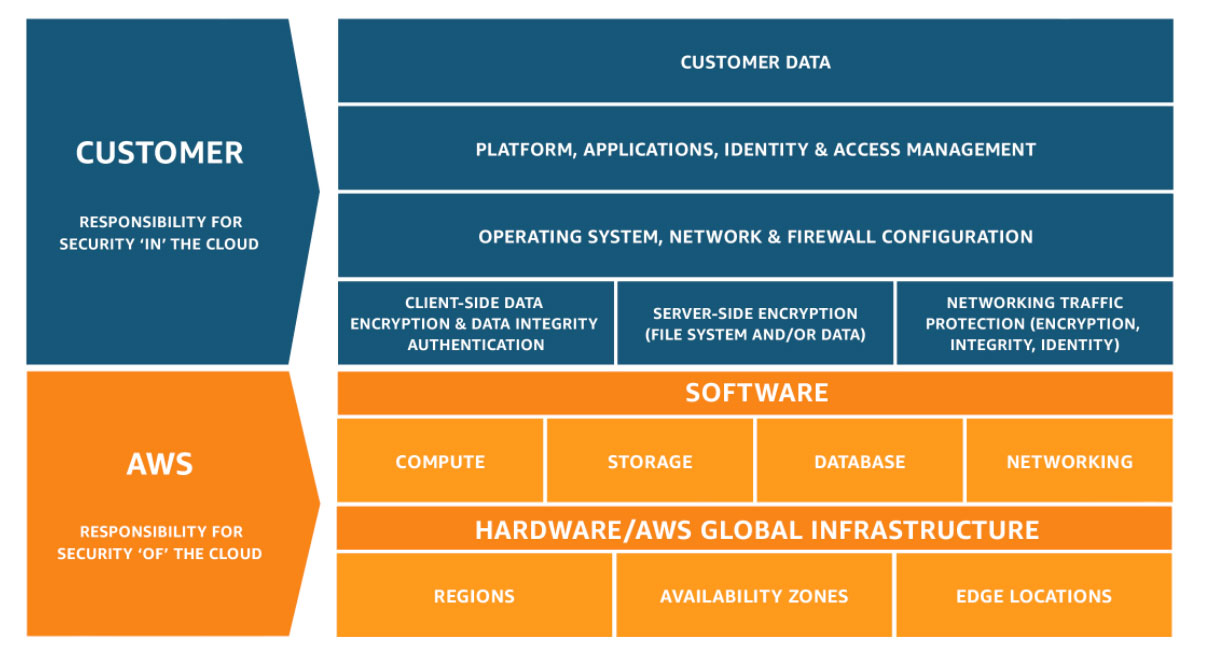
\includegraphics[width=1\textwidth]{aws-shared-responsibility.png}
        \caption{AWS Shared Responsibility Model}
    \end{figure}

    \newpage
    \subsubsection{Azure Shared Responsibility Model}
    \href{https://learn.microsoft.com/en-us/azure/security/fundamentals/shared-responsibility}{Azure Shared Responsibility Model}\footcite{site:azure-shared-responsibility-model} is a model that defines the responsibilities of Microsoft and the customer for security. The responsibility varies depending on wheter the service is \textit{Software as a Service} (SaaS), \textit{Platform as a Service} (PaaS), \textit{Infrastructure as a Service} (IaaS) or on premise. Regardless of the deployment type, the customer always detain data, endpoints account and access management responsibilities.\\
    
    \begin{figure}[htbp]
        \centering
        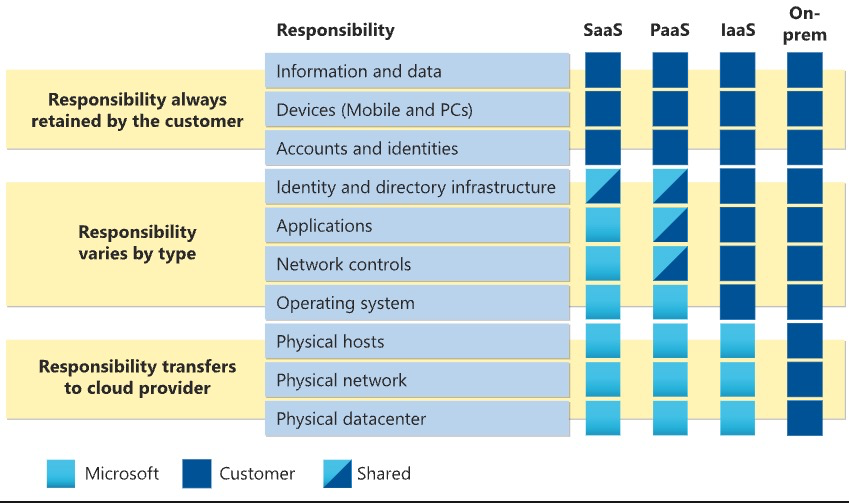
\includegraphics[width=1\textwidth]{azure-shared-responsibility.png}
        \caption{Azure Shared Responsibility Model}
    \end{figure}

\section{Scalability}
The system must be able to scale horizontally and vertically. The system must be able to handle a large amount of data and must be able to automatically scale to handle more data. Fully managed services and autoscaling properties offered by the cloud providers can be used to handle the scaling of the system.
